\documentclass[10pt,journal,compsoc]{IEEEtran}
\usepackage[brazilian]{babel}
\usepackage[utf8]{inputenc}
\usepackage{graphics}

\usepackage{minted}
\usepackage{xcolor}
\definecolor{LightGray}{gray}{0.9}
\definecolor{DarkGray}{gray}{0.1}
\usemintedstyle{monokai}


\begin{document}

\title{Password Leak \\ Processamento Paralelo}
\author{André~Thiago~Borghi~Couto,~\IEEEmembership{Graduando,~UFES}
\IEEEcompsocitemizethanks{\IEEEcompsocthanksitem A.T.B. Couto é graduando em ciência da computação, na UFES, campus CEUNES, em São Mateus - ES.\protect\\
E-mail: andreww.max@hotmail.com
}
\thanks{Trabalho escrito em 9 de junho de 2019;}}
\markboth{\LaTeX\ UFES - Processamento Paralelo,~Vol.~1, EP.~1, Junho~2019}
{Couto \MakeLowercase{\textit{et al.}}: Estudo de paralelização de busca em arquivos}

\IEEEtitleabstractindextext{
\begin{abstract}
% Em computação quando temos que pensar em um exemplo simples de aplicação, diversas formas, métodos, processos podem ser lembrados para demonstração do quão melhor e rápida pode ser a computação, apresentando a um leigo, provavelmente qualquer exemplo seria útil, e para nós? Como estudantes de computação devemos ter uma resposta simples e objetiva para o representar o potencial de nossos esforços, neste trabalho, discutiremos algumas técnicas e resultados de nosso problema mais tradicional, a busca.
In computing when we have to think of a simple example of application, various forms, methods, processes can be remembered to demonstrate how better and faster computing can be, presenting a layman, probably any example would be useful, and for us? As computer students we must have a simple and objective answer to represent the potential of our efforts, in this paper we will discuss some techniques and results of our more traditional problem, the search.
\end{abstract}

\begin{IEEEkeywords}
Computer Science, Computational Search, Parallel Programming, \LaTeX, Ciência da Computação, Threads, Busca Binária, Hash, Busca, Pragramação Paralela.
\end{IEEEkeywords}}

\maketitle
\IEEEdisplaynontitleabstractindextext
\IEEEpeerreviewmaketitle
\IEEEraisesectionheading{
    \section{Introdução ao Problema}
        \label{sec:introduction}}

\IEEEPARstart{E}{sse} é um problema clássico da computação: Busca.
A forma mais natural de resolver esse problema é comparar a senha buscada com cada uma das senhas vazadas (busca sequencial). 
Esse algoritmo possui complexidade O(n). Considerando que serão feito m buscas, então a implementação terá complexidade O(mn).
Uma forma de melhorar a complexidade do algoritmo é ordenar os dados e usar uma busca binária (O(m log n)).
No entanto, temos o custo computacional para ordenar os dados.

Será que ao paralelizar a busca sequencial, conseguimos um tempo de execução melhor que a busca binária?
Sim, até a busca do arquivo de 500 senhas o desempenho da busca sequencial paralelizada é melhor ou próximo à busca binária.

Para isso, precisamos de quantas threads?
Devido à ordenação do Vector temos uma perda de desempenho considerável para pequenas quantidade, então a busca binária é mais lenta até mesmo que a busca sequencial, mas com as threads, o desempenho é grande começando com apenas 2, já temos muita vantagem.

Para qual tamanho de n e m?
Basicamente temos o n fixo para todas as buscas que é 10'000'000, então a mudança ocorre no m, que as threads tem melhor desempenho nos 1, 2, 100, 500. 
	
Ou será que ordenar os dados não traz vantagens?
Ordenar os dados é crucial para o melhor desempenho e funcionamento da busca binária, então é de suma importância que a ordenação também faça parte da contagem do tempo gasto para execução do código.


\section{Estratégia}
Para começar, temos o armazenamento em memória que irá carregar todas as informações dos arquivos a serem usados no programa, para isto utilizamos a biblioteca Vector<> do C++, junto com uma função simples de leitura de arquivos, onde criamos o arquivo com as senhas lidas, usado para as senhas vazadas e as verificadas, retornando o vetor preenchido.

\begin{listing}[ht]
\begin{minted}[frame=lines, bgcolor=DarkGray, fontsize=\footnotesize, framesep=2mm, baselinestretch=1.2]{c}

vector<string> sVazadas, sVerificar, sEncontradas;

vector<string> lerSenhas(FILE *arq){
    vector<string> senhas;
    char *senha = (char *) calloc(50, sizeof(char));

    while(EOF != fscanf(arq, "%s", senha)) 
        senhas.push_back(senha);

	return senhas;
}
\end{minted}
\caption{Leitura dos arquivos de senhas}
\label{listing:1}
\end{listing}

Os Vectors<> são globais, logo não é necessário passá-los para as funções, simplificando e padronizando os demais arquivos que são utilizadas threads, então agora devemos ver que o objetivo dos códigos é otimizar o desempenho da busca, ao analisarmos o código sequencial temos o núcleo central da busca no seguinte trecho:

\subsection{Busca Sequencial}
\begin{listing}[ht]
\begin{minted}[frame=lines,bgcolor=DarkGray, fontsize=\footnotesize, framesep=2mm, baselinestretch=1.2]{c}
bool buscaElementoUnico(string ver){
    for (int j = 0; j < sVerificar.size(); j++)
        if(!ver.compare(sVerificar[j]))
            return true;
    return false;
}

void buscaElemento() {
    for (int i = 0; i < sVazadas.size(); i++)
        if(buscaElementoUnico(sVazadas[i]))
            sEncontradas.push_back(sVazadas[i]);
}
\end{minted}
\caption{Busca Sequencial}
\label{listing:2}
\end{listing}

Esse trecho representa a busca em si, onde temos a função buscaElemento(), que percorre o Vector das senhas Vazadas, e então faz a chamada da função buscaElementoUnico(), passando a senha a ser verificada, dentro desta função temos outro loop, para percorrer o Vector de senhas Verificadas, que por sua vez a senha Vazada é comparada à todas as senhas a serem Verificadas, com essa ideia vemos que todas serão comparadas à todas, e dentro da função, para evitar desperdício de comparações, o retorno ajuda no desvio, quando é encontrada a senha à ser verificada, com o retorno da senha encontrada, temos a inserção da senha em um Vector de resultado, que armazena as senhas encontradas. Após todas as senhas a serem verificadas e processadas, e devidamente armazenadas (caso encontradas) a execução do programa termina, exibindo o tempo gasto com a busca das senhas.


\subsection{Busca Sequencial Paralelizada}
	
\begin{listing}[ht]
\begin{minted}[frame=lines,bgcolor=DarkGray, fontsize=\footnotesize, framesep=2mm, baselinestretch=1.2]{c}
int N, numThreads, ind;
mutex mux;

bool buscaElementoUnico(string ver){
    for (int i = 0; i < sVerificar.size(); i++)
        if(!ver.compare(sVerificar[i]))
            return true;
    return false;
}

void buscaElemento(int ini, int fim) {
    for (int i = ini; i < fim; i++){
        if(buscaElementoUnico(sVazadas[i])){
            mux.lock();
            sEncontradas.push_back(sVazadas[i]);
            mux.unlock();
        }
    }
}

void execThread(){
    thread th[numThreads];
    ind = 0;
    for (int i = 0; i < numThreads; i++){
        int ini, fim;
        if (i == numThreads - 1){
            ini = ind;
            fim = N;
        } else {
            ini = ind;
            fim = ind + N / numThreads;
            ind += N / numThreads;
        }
        th[i] = thread(buscaElemento, ini, fim);
    }	
    for (int i = 0; i < numThreads; ++i)
        th[i].join();
}
\end{minted}
\caption{Busca Sequencial Paralelizada}
\label{listing:3}
\end{listing}

	A função execThread(), basicamente, utiliza os valores das entradas (SenhasVazadas, SenhasVerificadas e numero de Threads) para cálcular os limites entre as threads que serão utilizadas. O código paralelo, com as modificações necessárias para adição de threads, que são variáveis de armazenamento global (N, numThreads, ind e mux), representam numero quantidade de senhas, quantidade de threads, uma variável para controle do cálculo da divisão de valores das threads e o semáforo mutex utilizado ao decorrer do código, e como proposto temos detalhes que ao invés de percorremos o Vector de senhas a serem verificadas, percorremos o de senhas Vazadas, pois os limites devem ser passados para cada thread, com o intuito de diminuir o campo de repetições inúteis, logo temos a divisão de threads, para a comparação com a função buscaElementoUnico(), retornado ao encontrar uma senha uma senha verificada. Um detalhe importante é que ao chamar a função buscaElementoUnico(), que é booleana, encadeada na estrutura do IF, se for verdadeira temos a inserção da senha no Vector de encontradas, dentro dessa estrutura condicional temos um semáforo, para controlar a escrita da função que adiciona as senhas encontradas, com o mutex.lock() e consequentemente, mutex.unlock(). Após todas as senhas serem processadas e armazenadas (caso encontradas) a execução do programa termina, exibindo o tempo gasto com a busca das senhas.


\subsection{Busca Binária Sequencial}

\begin{listing}[ht]
\begin{minted}[frame=lines,bgcolor=DarkGray, fontsize=\footnotesize, framesep=2mm, baselinestretch=1.2]{c}
bool BSTRecursiva(int inicio, int fim, string ver) {
    if (inicio <= fim) {
       int meio = (inicio + fim) / 2;
       if (!ver.compare(sVazadas[meio])){ 
           return true;
       } else if (ver.compare(sVazadas[meio]) > 0){
           return BSTRecursiva(meio + 1, fim, ver);
       } else { 
           return BSTRecursiva(inicio, meio-1, ver);
       }
    }
    return false;
}

void buscaElemento(int ini, int fim) {
    for (int i = 0; i < sVerificar.size(); i++)
        if(BSTRecursiva(ini, fim, sVerificar[i]))
            sEncontradas.push_back(sVerificar[i]);
}

int main(int argc, char *argv[]){
    ....
    ....
    sort(sVazadas.begin(), sVazadas.end());
    sort(sVerificar.begin(), sVerificar.end());
    ....
    ....
}
\end{minted}
\caption{Busca Binária Sequencial}
\label{listing:4}
\end{listing}

	A busca binária tem um método diferente dos anteriores por utilizar uma busca parcial, sem a comparação de todas as senhas, logo obtendo mais desempenho, porém uma desvantagem é que necessita da ordenação do vetor para a busca ser efetiva, então existe um gasto computacional extra considerável (declarado na main()). Dentre as funções temos a buscaElemento(), que faz a divisão das senhas vazadas e executa a função BSTRecursiva() para cada senha a ser verificada, essa função recebe os limites de busca, onde utiliza-os para identificar o intervalo que ira fazer a busca, o cálculo é feito antes das comparações, comparações essas que identificam a posição relativa ao centro, que foi obtida no cálculo, então caso não seja a chave central, temos o desvio para a direção que a chave pode estar, recursivamente, até a identificação ou não da senha verificada. Se a função buscaElementoUnico(), que é booleana, for verdadeira temos a inserção da senha no Vector de encontradas, e a próxima senha é verificada, até o fim. Após todas as senhas serem processadas e armazenadas (caso encontradas) a execução do programa termina, exibindo o tempo gasto com a busca das senhas.


\subsection{Busca Binária Paralelizada}
	
	Esta busca binária é uma mesclagem das implementações de busca binária sequencial e busca sequencial paralelizada, discutidas anteriormente, como as estratégias já foram discutidas, temos apenas detalhes, locais que foram feitas as devidas adaptações, como na função execThread() que recebeu o código de ordenação (sort), e também para o vetor poder ser utilizado na busca binária e o semáforo que foi adicionado ao trecho da condicional que executa a BSTRecursiva(), organizando as inserções no Vector de senhas encontradas.


\subsection{Busca Hash}
	
\begin{listing}[ht]
\begin{minted}[frame=lines,bgcolor=DarkGray, fontsize=\footnotesize, framesep=2mm, baselinestretch=1.2]{c}
unordered_map<string, unsigned long long int>
                       lerSenhasVazadas(FILE *arq){
    unordered_map<string, unsigned long long int> 
                                            senhas;
    hash<string> senhaHash;
    char *senha = (char *) calloc(50, sizeof(char));
    while(EOF != fscanf(arq, "%s", senha)) {
        string s(senha);
        senhas[s] = senhaHash(s);
    }
    return senhas;
}

void buscaElemento() {
    hash<string> senhaHash;
    for (int j = 0; j < sVerificar.size(); j++){
        string s(sVerificar[j]);
        if(!(sVazadas.find(s) == sVazadas.end()))
            sEncontradas.push_back(sVerificar[j]);
    }
}
\end{minted}
\caption{Busca Tabela Hash}
\label{listing:5}
\end{listing}
	
	Este outro código, utilizando tabela Hash, curiosamente não faz parte do trabalho, temos a mesma intenção de busca de senhas, pelo método a ser usado temos algumas diferenças dos anteriores, então primeiramente temos que gerar a tabela com as senhas e seus Hash's, logo o tipo utilizado foi unordered\_map$<>$, que  faz a combinação de mapeamento entre tipos, como uma estrutura, então para cada entrada String temos o cálculo do Hash respectivo, e por fim a inserção no unordered\_map$<>$, finalizando a inserção.
	Como a ideia da tabela Hash, é obter o índice que se encontra a informação instantaneamente temos apenas que pegar a senha a ser verificada e calcular seu Hash, obtendo assim o índice da senha, caso a senha realmente exista, temos a adição dela no Vector de encontradas, realizando esse processo até a última. O tempo é extremamente otimizado. 
	

\section{As configurações do computador utilizado}
Os códigos foram implementados em C++ e compilados com GNU g++ versão 7.3.0, com a opção -O3 ativada.
Os experimentos foram realizados em uma máquina Intel(R) Core(TM) i7-5500U CPU @ 2.40GHz, com os caches de: L1d - 32K, L1i - 32K, L2 - 256K, L3 - 4096K. Tendo 8 GB de memória RAM e com S.O. Linux Mint 19.

\begin{figure}[!ht]
	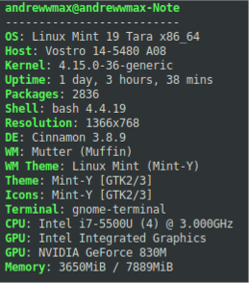
\includegraphics{Config.png}
	\caption{Neofetch}
	\label{fig_sim}
\end{figure}

\section{Experimentos e Gráficos}
Com a execução dos códigos nas restrições do trabalho, em que para gerar os gráficos foram repetidas 15 vezes cada código, logo temos a media e o desvio padrão nos gráficos.
Analisando cada gráfico temos algumas considerações a serem feitas, no geral o resultado esperado foi o obtido, com exceção dos códigos de busca binária, que após revisar e fazer testes pontuais, com novas senhas, geradas apenas para teste, em um bloco selecionado, descobri que a quantidade entre 75 e 200 temos um grande desvio de tempo, dificilmente seria descoberto, caso não se aplica-se novos testes com diferentes quantidades, então após a analise de quantidade (todos os arquivos de senhas verificadas, com os 75 e 200), algoritmos (recursivo e iterativo), divisões (em Threads), conclui que o código em si, não tem problema, mas um detalhe mais profundo na implementação pra deter erros, o semáforo, assim como esperado, do mutex, temos a seleção da sequencia que ira ser inserido, devido a quantidade baixa quantidade de senhas verificadas, temos uma rápida resposta de encontrado, logo ao travar a chance de uma outra thread também ter encontrado é alta, podemos concluir que o semáforo que é essencial para o funcionamento, então o tempo sofre essa pequena alteração.

Seguindo os gráficos, os resultados coerentes com o esperado, sendo:
O código sequencial é mais lento que os todos os outros, exceto no código paralelizado com 1 (uma) thread, a partir do arquivo com 100 senhas verificadas, aumentando exponencialmente o tempo nos próximos arquivos. A exceção que é o código com 1 thread, tem o pior desempenho pelo processo de cálculo e criação da thread.
O código paralelizado tem seus objetivos alcançados, que é dividir as tarefas entre as threads, logo com os gráficos, que nos apresentam tempos reduzidos à medida que a quantidade de senhas verificadas, além da relação de threads, a limitação de hardware, traz resultados pouco reveladores, no qual a execução com 8 threads, obteve quase exatamente o mesmo tempo da execução com 4 thread, sabendo que as threads não suportadas fisicamente ficam em concorrência durante a execução, talvez piorando ou não o desempenho, mesmo sabendo que é inútil deixar essas threads executando e sendo trocadas o tempo todo, até o fim do programa.
O código com a busca binária temos uma grande diferença, pois temos a ordenação durante a execução, logo isso entra como tempo quase constante na execução de todos os modos de execução, então temos a consistência do resultado, que faz jus a classificação de O(m log n), sendo resultados constantes, o código não faz uma curva de elevação enquanto a quantidade de senhas verificadas aumenta, pelo fato de serem números inteiros, e pares, não sendo possível o cálculo do elemento médio entre 2, o piso sempre o coloca à esquerda ou direita, sendo assim, sempre será uma folha, em analogia a árvore de busca binária, gerando um resultado quase que linear entre todas as execuções.
O código de busca binária paralelizada, foi de pouca importância, apesar de não apresentar desempenho superior ao sequencial, por falta de análise de minha parte, que foi difícil perceber que não estava criando novas threads ao executar.
O código extra implementado com Hash, que obteve bons resultados, se considerarmos o núcleo, pois o gasto computacional para a criação do unordered\_map e adição do Hash, é alto e deixa o tempo total do programa em desvantagem aos códigos que são diretamente comparativos, sendo executado em O(1).

No geral temos uma análise que ao executarmos uma pequena quantidade de senhas para verificá-las temos um melhor desempenho que é obtido por apenas fazer uma simples repetição, não sendo vantajoso para grandes quantidade. Mesmo ao paralelizarmos essa busca sequencial, com números muito altos temos um grande aumento do tempo, então o que nos resta é observar e entender que a grades quantidades a busca linear, não traz vantagens, e ao aumentarmos o número de verificações códigos como busca binária tornam-se eficientes, ao ignorar muitas das comparações antes de achar o resultados. A tabela Hash, por sua vez não utiliza dos métodos de comparação anteriores, então temos uma reação direta.
	
A seguir algumas das perguntas à serem respondidas, pela descrição do trabalho:
Considerando a busca sequencial, a partir de que quantidade de senhas é mais vantajoso paralelizar? E considerando a busca binária?
A partir de 100 senhas à serem verificadas, temos que paralelizar para obter melhor desempenho, já com a busca binária será melhor com números acima de 500. 

Considerando a busca sequencial, a partir de quantos threads o tempo não diminui consideravelmente? E considerando a busca binária?
A partir de 4 threads, que neste caso sabemos que é devido à concorrência sobre o hardware, que no caso do meu PC é 2 núcleos com 2 threads cada, então cada thread adicionada acima desse valor torna a melhoria do desempenho pouco provável. Já com busca binária é mais eficiente a partir das 500 senhas à serem verificadas, levando em conta todo o processo de ordenação.

Considerando o número máximo de threads do computador utilizado, teve algum caso em que a implementação paralelo que usa o busca sequencial foi melhor que a que usa a busca binária?
Utilizando 4 threads, o máximo do meu PC, o desempenho do código paralelo, é melhor até os arquivos com 100 senhas, os demais resultados são vantagem para a busca binária.
	
Em outro tipo de análise, obtive resultados sobre a memória, utilização e consumo, que são representados a seguir, com um modelo de execução padrão sendo visto na lista de comandos \ref{listing:6}

\usemintedstyle{vim}
\begin{listing}[ht]
\begin{minted}[frame=lines, bgcolor=LightGray, fontsize=\footnotesize, framesep=2mm, baselinestretch=1.2]{shell}
env time -f "%C\n\tTempo de Execução:
            %E\n\tMemória usada: %M\n"
            -o memory.txt -a 
            ./EP1......... 0 
            txt/SenhasVazadas.txt txt/1000.txt

./EP1Seq 0 txt/SenhasVazadas.txt txt/1000.txt
    Tempo de Execução: 0:36.17
    Memória usada: 1051808

./EP1Paralel 4 txt/SenhasVazadas.txt txt/1000.txt
    Tempo de Execução: 0:19.84
    Memória usada: 1051772

./EP1BSTSeq 0 txt/SenhasVazadas.txt txt/1000.txt
    Tempo de Execução: 0:11.28
    Memória usada: 1051940

./EP1BSTParalel 4 txt/SenhasVazadas.txt txt/1000.txt
    Tempo de Execução: 0:10.88
    Memória usada: 1052048

./EP1Hash 0 txt/SenhasVazadas.txt txt/1000.txt
    Tempo de Execução: 0:09.86
    Memória usada: 1373080

\end{minted}
\caption{Resultados do teste de consumo de memória}
\label{listing:6}
\end{listing}

Assim com os dados obtidos, temos o consumo básico de memória entre todos os códigos, Sequencial, Paralelizado, Busca Binária e Busca Binária Paralelizada. Porém o código de Hash sai com uma grande margem acima dos demais, utilizando mais memória, isso seria um problema, em questão de entrada de dados de maior magnitude. 

Podemos concluir então que para pequenas quantidades usamos busca sequencial paralelizada, à medida que aumentamos o número de comparações escolhemos a busca binária, e se tivermos uma disponibilidade de hardware sem grandes problemas e que precisaremos de extrema eficiência nos resultados, em redução de tempo de execução, escolhemos a Tabela Hash.


%%%%%%%%%%%%%%%%%%%%%%%%%%%%%%%%%%%%%%%%%%%%%%%%%%%%%%%%%%%%%%%%%%%%%%%%%%%%%%%%%%%%%%
\appendices
\section{Gráfico Comparativo Sequencial e Paralelo}
\begin{figure}[!t]
	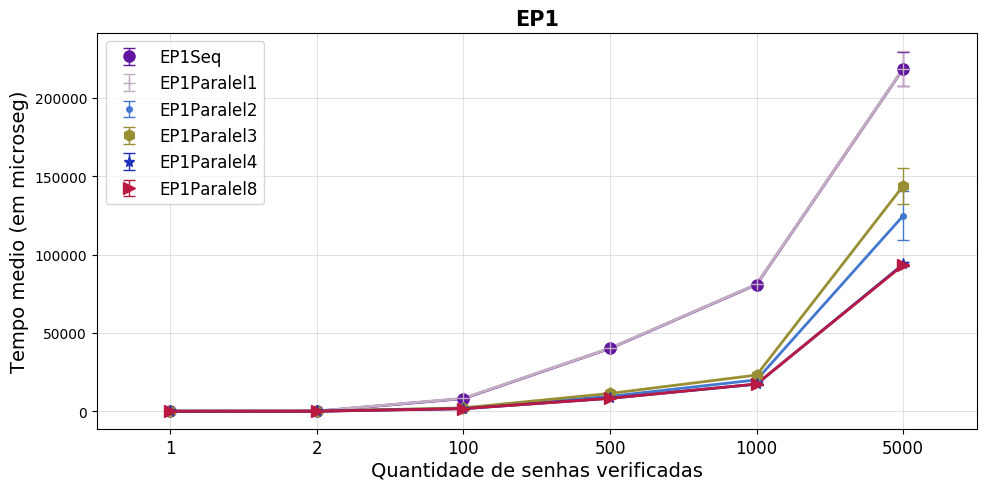
\includegraphics{GraficoEP1-Seq-Par-Nucleo.png}
	\caption{Gráfico com apenas o tempo do núcleo de busca}
	\label{figSeqNucleo}
\end{figure}
\begin{figure}[!t]
	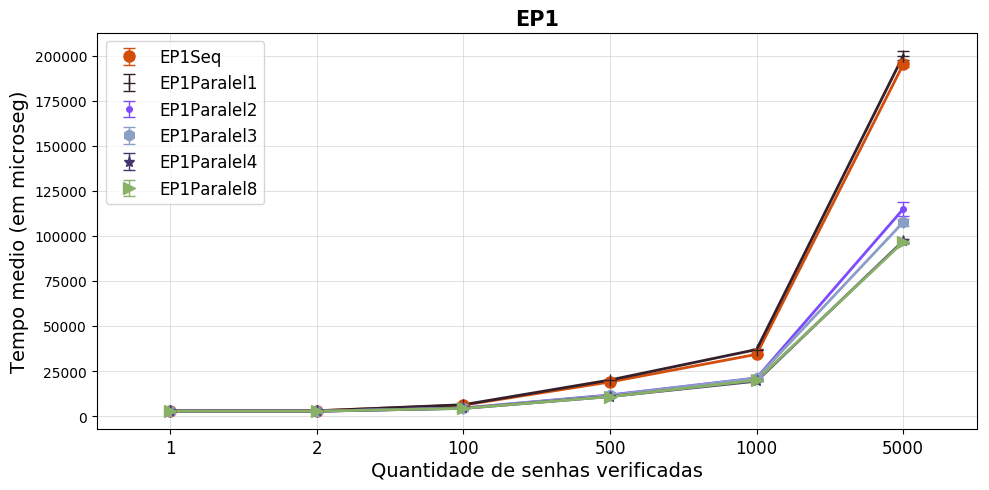
\includegraphics{GraficoEP1-Seq-Par-Total.png}
	\caption{Gráfico com o tempo do total de execução}
	\label{figSeqTotal}
\end{figure}
\newpage

\section{Gráfico Comparativo Busca Binária Sequencial e Paralelo}
\begin{figure}[!t]
	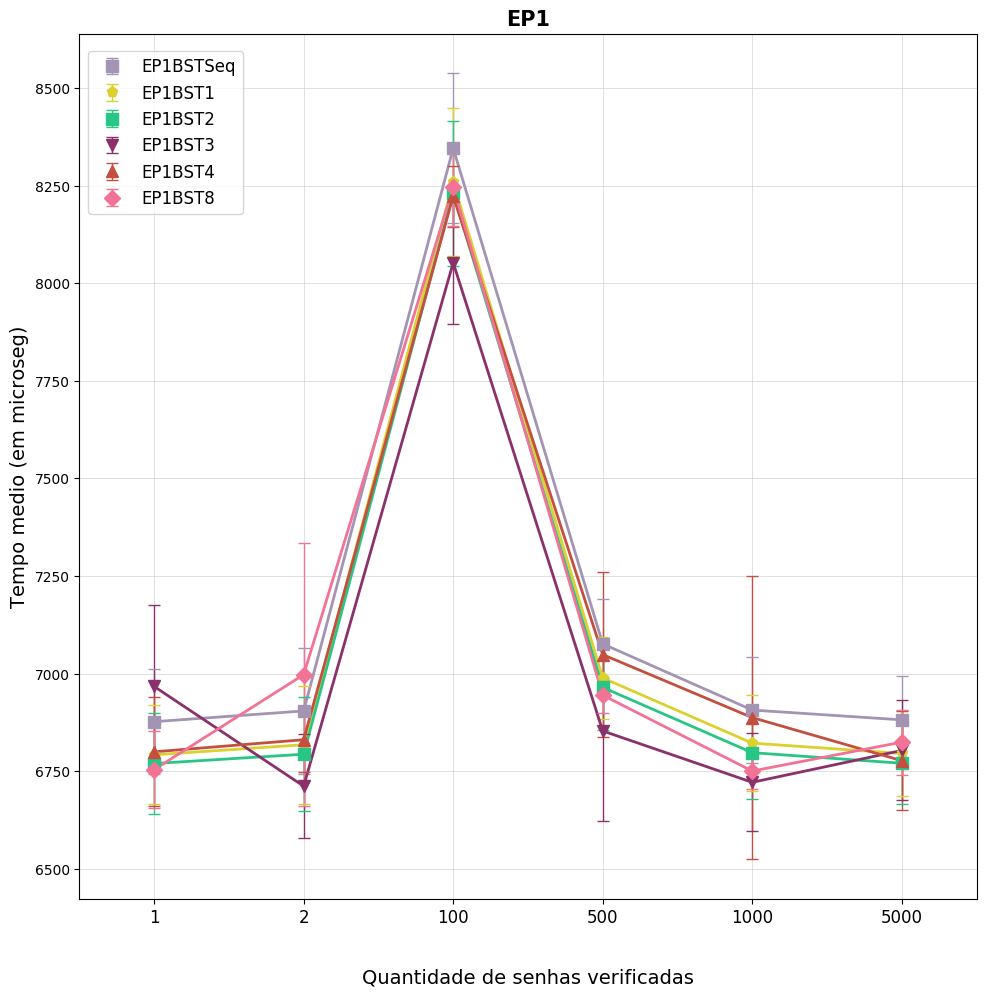
\includegraphics{GraficoEP1BSTNucleo.png}
	\caption{Gráfico com apenas o tempo do núcleo de busca}
	\label{figSeqNucleo}
\end{figure}
\begin{figure}[!t]
	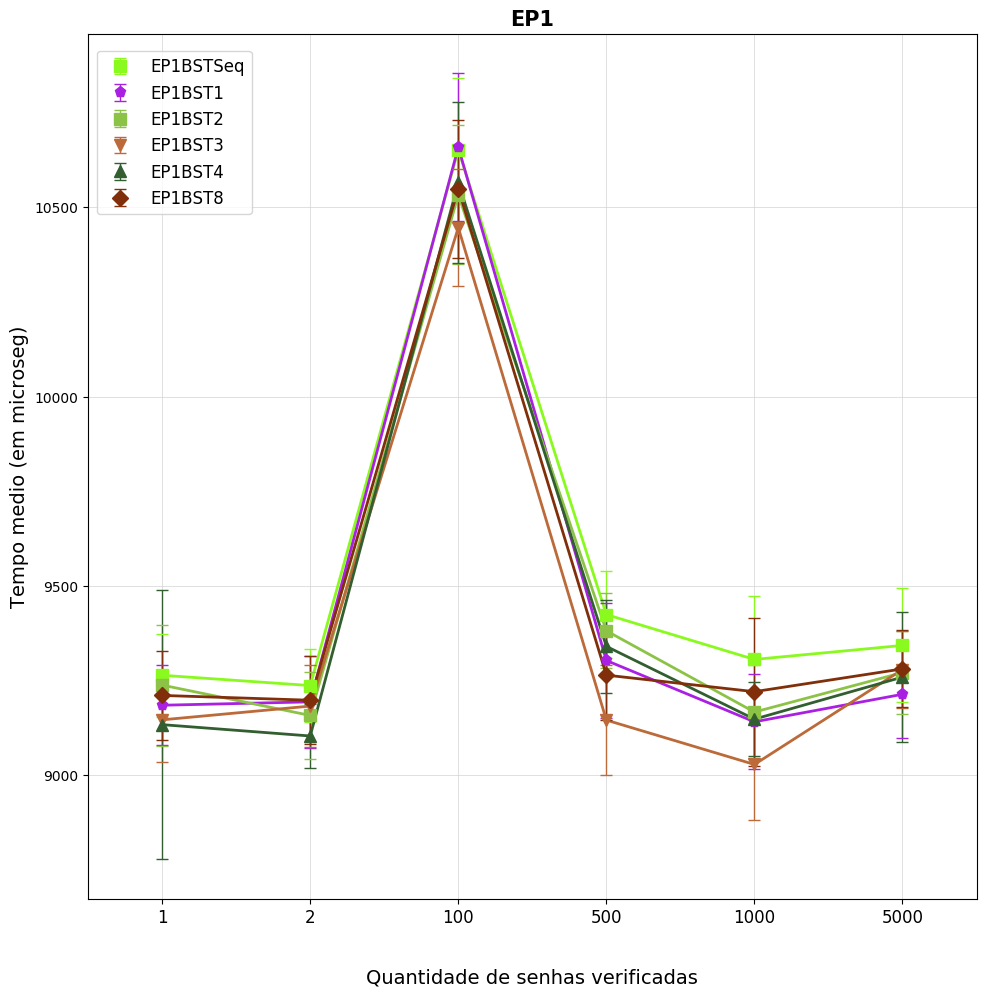
\includegraphics{GraficoEP1BSTTotal.png}
	\caption{Gráfico com o tempo do total de execução}
	\label{figSeqTotal}
\end{figure}

\section{Gráfico de todas as opções reunidas}
\begin{figure}[!t]
	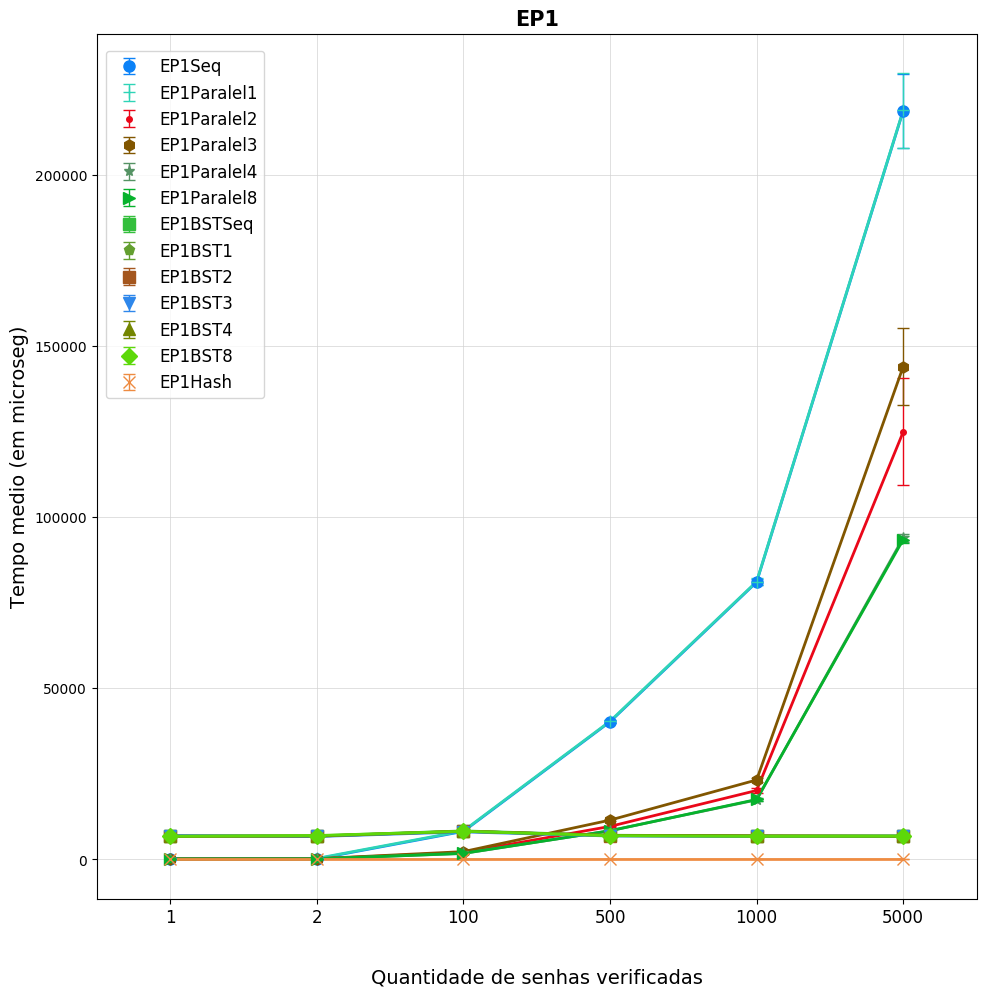
\includegraphics{GraficoEP1CompletoNucleo.png}
	\caption{Gráfico com apenas o tempo do núcleo de busca}
	\label{figCompNucleo}
\end{figure}
\begin{figure}[!t]
	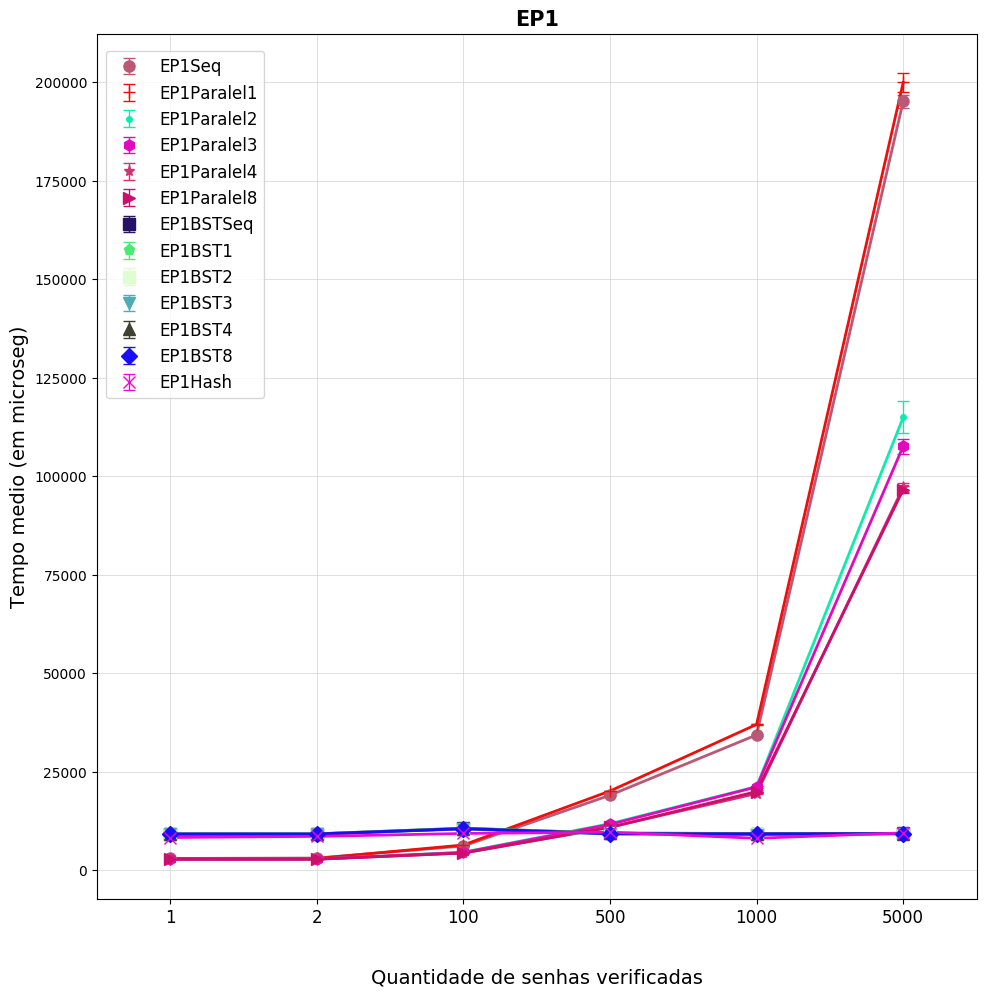
\includegraphics{GraficoEP1CompletoTotal.png}
	\caption{Gráfico com o tempo do total de execução}
	\label{figCompTotal}
\end{figure}

%%%%%%%%%%%%%%%%%%%%%%%%%%%%%%%%%%%%%%%%%%%%%%%%
% \begin{IEEEbiography}{André Thiago Borghi Couto}
% atualmente cursa graduação em Engenharia da Computação (2016/1) na Universidade Federal do Espírito Santo. Possui conhecimento em desenvolvimento de software, banco de dados, projetos em Arduino, design gráfico e tem interesse nos temas de automação em Arduino, inteligência artificial, redes de computadores e processamento de imagens.
% \end{IEEEbiography}

\begin{IEEEbiographynophoto}{André Thiago Borghi Couto}
atualmente cursa graduação em Engenharia da Computação (2016/1) na Universidade Federal do Espírito Santo. Possui conhecimento em desenvolvimento de software, banco de dados, projetos em Arduino, design gráfico e tem interesse nos temas de automação em Arduino, inteligência artificial, redes de computadores e processamento de imagens.
\end{IEEEbiographynophoto}


\end{document}